\chapter{Introduction to relevant topics}
Graphene is a two-dimensional lattice of carbon atoms, arranged in a honeycomb structure as shown in the figure \ref{fig:graphene} Although it is straightforward to build many layers of these lattices (a substance known as graphite), it was long thought that a purely two-dimensional lattice would be unstable to thermal fluctuations and impossible to create.
This changed in 2004 when Andre Geim and Konstantin Novoselov succeeded in isolating two-dimensional graphene \cite{firstExfoliation}. For this, they won the 2010 Nobel prize. As we now show, the band structure of graphene is particularly interesting.
\begin{figure}[h]
    \makebox[\textwidth][c]{
        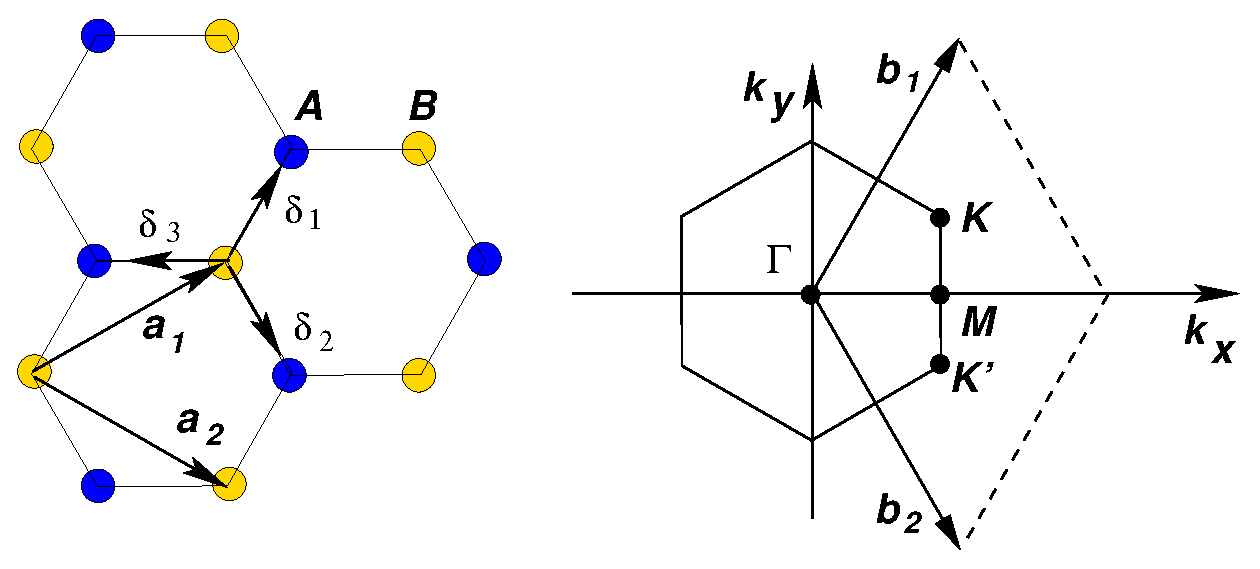
\includegraphics[width=\linewidth]{Immagini/graphene/structure.eps}
        }%
    \caption{On the left there is the lattice structure of graphene made out of two interpenetrating triangular lattices ($a_1$ and $a_2$ are the lattice unit vectors, and $\mathbf \delta_{i}$ with $i\in {1,2,3}$ are the nearest neighbors. On the right the corresponding Brillouin zone, the Dirac cones are located at the $K_0$ and $K_1$ points) \cite{guinea2008review}}
    \label{fig:graphene}
\end{figure}\\
We define the primitive lattice vectors $\vect a_1$ and $\vect a_2$ as follows:
\begin{equation}
    \vect a_1=\frac{a}2
    \begin{bmatrix}
        3 \\ \sqrt 3
    \end{bmatrix}\quad \quad
    \vect a_2=\frac{a}2
    \begin{bmatrix}
        3 \\ -\sqrt 3
    \end{bmatrix}
\end{equation}
Where $a$ is the distance between two neighboring atoms, which in graphene is $\approx 1.4\times 10^{-10}$m. The sublattice A is defined as all the points $r = n_1\vect a_1 + n_2\vect a_2$ with $n_i \in \mathbb Z$ (yellow in figure \ref{fig:graphene}), sublattice B is defined as all points $r = n_1\vect a_1 + n_2\vect a_2 + \delta$ with $\delta = (a, 0)$ (blue in figure \ref{fig:graphene}). These are the white dots.

The reciprocal lattice vectors $\vect b_i$ are the vectors that satisfy $\vect a_i\cdot \vect b_j=\delta_{ij}$ and are equal to 
\begin{equation}
    \vect b_1=\frac{2\pi}{3a}\begin{bmatrix}
        1 \\ \sqrt 3
    \end{bmatrix}
    \quad \quad
    \vect b_2=\frac{2\pi}{3a}\begin{bmatrix}
        1 \\ -\sqrt 3
    \end{bmatrix}
\end{equation}
This reciprocal lattice is also triangular. The Brillouin zone is constructed in the usual manner by drawing perpendicular boundaries between the origin and each other point in the reciprocal lattice giving rise to a hexagonal Brillouin zone with $K_0$ and $K_1$ as the vertices of the hexagon, where 
\[
    K_0=\frac 13 (2b_1+b_2)\quad \quad K_1=\frac 13 (b_1+2b_2)
\]

\begin{equation}
    K_0=\frac{2\pi}{3a}\left(1,\frac 1{\sqrt 3}\right)\quad\quad K_1=\frac{2\pi}{3a}\left(1,-\frac 1{\sqrt 3}\right)
\end{equation}

\subsubsection*{The tight binding approach}
To investigate the band structure of graphene, we are going to use the tight binding approach \cite{bloch1929quantenmechanik}.
First we write the Hamiltonian.
\begin{equation}
    H=\frac{\vect p^2}{2m} + \sum_{\vect R\in C}V(x-\vect R)
    \label{eq:blochhamiltonian}
\end{equation}
where the set $C=\left\{n_1\vect a_1 +n_2\vect a_2 + j\boldsymbol \delta\,|\,n_1,n_2\in \mathbb Z,\, j\in \{0,1\} \right\}$ is the set of all the positions of the atoms.

Let $\ket{n,\vect R}$ be the $n$-th eingenstate of the Hamiltonian of a carbon atom placed in $\vect R$.
Due to translational symmetry, the wave function must satisfy the Bloch theorem, this tells us that the eingenstates of the Hamiltonian can be written as
\begin{equation}
    \ket{n,\vect k}=\sum_{\vect R\in C} e^{i\vect k \cdot \vect R}\ket{n,\vect R}
\end{equation}
With this we can now calculate the matrix elements of the Hamiltonian
\begin{equation}
    \big\langle n,\vect k\big|H\big| n',\vect k'\big\rangle=
    \sum_{\vect k\vect k',\vect R\vect R'}e^{i\vect k\cdot \vect R-i\vect k'\cdot\vect R'}
    \big\langle n,\vect R\big|H\ket{n',\vect R'}
\end{equation}
Since the right-hand side of the summation does not depend on $k$ we have that the terms with $k\neq k'$ are equal to zero. So the equation above becomes
\[
    \big\langle n,\vect k\big|H\big| n',\vect k'\big\rangle= \big\langle n,\vect k\big|H\big| n',\vect k\big\rangle\delta_{\vect k,\vect k'}
\]
Ok, now we need to calculate $ \big\langle n,\vect R\big|H\ket{n',\vect R'}$. Using equation \ref{eq:blochhamiltonian} we get that if $\vect R=\vect R'$
\begin{equation}
    \big\langle n,\vect R\big|H\ket{n',\vect R}=E_n\delta_{n,n'}+
    \underbrace{
        \sum_{\vect R'\neq \vect R}
        \big\langle n,\vect R\big|V(r-\vect R')\ket{n',\vect R}
    }_{\text{small}}
    \label{eq:tight1}
\end{equation}
The second term is much smaller than the first one, so we can ignore it.\\
In the case where $\vect R$ and $\vect R'$ are two nearest neighbors we have that $\vect R'=\vect R+\boldsymbol\delta_i$ with $i\in \{1,2,3\}$ (fig. \ref{fig:graphene}).\\ We can expand the state localized in $\vect R'$ in terms of the ones localized in $\vect R$

\begin{equation}
    \ket{n',\vect R +\boldsymbol\delta_i}=
    \sum_{n''}\ket{n'',\vect R}\braket{n'',\vect R}{n',\vect R+\boldsymbol\delta_i}=
    \sum_{n''}\ket{n'',\vect R}t_{nn'}^1
\end{equation}
Where $t_{nn'}\equiv\braket{n,0}{n',\boldsymbol\delta_i}$
This means that 
\begin{equation}
    \big\langle n,\vect R\big|H\ket{n',\vect R'}=
    \sum_{n''}\bra{n,\vect R}H\ket{n'',\vect R}t_{n'n''}\approx
    E_n t_{nn'}^1
\end{equation}
where in the last step we used \ref{eq:tight1}
